\chapter{Implementation}
\label{Chapter:Implementation}
Having provided detail on the design stage of the project, this chapter of the report begins to look moving from concepts to implementation. The web application being built will provide a way of delivering Fidelis to multiple users across multiple devices rather than creating a separate application tailored to each platform. The following sections will look at the technologies used to implement the application, along with detailed information on algorithm and UI implementation.

\section{Technologies}
Building Fidelis required collating a number of technologies. The technologies used for implementation can be categorised into storage, processing and visualisation technologies, each of which are discussed below.

\subsection{Storage}
MySQL is an open source database management system used for managing data held in a relational database management system \cite{MySQL:Home}. It is the world's most popular open source database, being used by some of the largest and fastest-growing organisations including Facebook, Google and Adobe. The reasons behind the use of MySQL database are vast but the key factor is the ease with which a MySQL database can be setup and migrated. MySQL databases have existed for many years which has led to gradual improvements over time, and as a result of these improvements MySQL databases now guarantee stability, scalability and security \cite{MySQL:Why}. The longevity of MySQL database systems is another appealing aspect, and has meant that a wide range of third-party party tools are available to the developer for working with and processing the data. 

\subsection{Processing}
Majority of the data processing will be done using PHP. All PHP scripts are executed on the server which may produce output that can be presented to the user. The language is used by millions of websites and has for some time been  a popular scripting language for dynamic web development. This wide adoption of the PHP scripting language has allowed extensive libraries and frameworks to be made available and used for rapid development of web applications. One such framework, Laravel, will be used to implement the MVC approach discussed in Chapter \ref{Chapter:Research}. PHP has shown to be scalable as it is powerful enough to be at the core of the biggest blogging system on the web, known as WordPress, but at the same time it is deep enough to run the largest social network, Facebook\cite{W3Schools:PHP_Intro, Wiki:WordPress, Fastcompany:Facebook_PHP}. This means that in the future if the system is to grow large enough, it can easily be scaled as done so over time by the aforementioned examples. 

In addition to PHP, JavaScript will be used for some client-side data processing along with SQL which will be used to process data from the database before it is retrieved. Python will be used to process user data needed for content-filtering, abuse detection, recommendations and reputation scoring. Like PHP, Python is also executed on the server-side, reducing the amount of processing and computation required on the client-side. Python was chosen not only for its popularity, but again like PHP it provides an extensive range of libraries that can be used during development. Examples of these include Scikit-Learn \cite{scikit:home}, which provides a number of data mining and analysis tools, and \emph{NumPy} and \emph{pandas}, which are useful for data manipulation.

\subsection{Visualisation}
HTML is coupled with CSS to define page structure, and design the components on the page \cite{W3:HTML5, W3:CSS}. In addition to this, the Laravel blade engine is being used to make the generation of pages easier by splitting content up into views that can be extended by or rendered inside other views \cite{Laravel:Blade}. This encourages good practices by abstracting the system and enforcing modularity throughout. Using the blade enginge supported the idea of using component-driven design, discussed in Chapter \ref{Chapter:ProjectManagement}. Building views in a modular fashion enables development in the future to easily integrate new components and replace master views seamlessly to change the overall system appearance. Bootstrap is also used as an additional framework to make the pages more dynamic by providing visual interaction.

\subsection{Installation and Setup}
Many of the technologies being employed are not included by default on an ordinary machine. Thus, before development could be initiated, it was necessary to install and configure the required technologies. This section details the configuration process for the technologies used, along with any prerequisites for them.

\subsubsection{Initial Setup}
An Apache web server capable of interpreting PHP and rendering web pages was required for development. In addition to this, an SQL server was need to host the MySQL database. XAMPP, which provides an SQL and web server, was the solution chosen to handle both these cases. Both servers are automatically configured by the XAMPP package upon installation and are immediately ready to use out of the box. XAMPP provides an easy-to-use control panel from which servers can be started, and accessing through \textit{http://localhost/}. Any files can them be placed inside the \textit{htdocs} folder, created during the installation process.

\subsubsection{IDE and Laravel}
The Laravel framework was used to build Fidelis, but it is not readily available to download as an archive. Instead, composer - a package manager, was used for the installation of the framework. Using composer, new projects can be created using the \textit{laraval new project-name} command. Executing this command creates a new \textit{project-name} directory with all the necessary files and project dependencies. Updates and additional packages may be installed using composer and the included \textit{packages.json} file.

The PHPStorm IDE, developed by JetBrains, was used throughout the project for all web-related development. PHPStorm is a dedicated PHP IDE, and has the capability to include plugins providing features that enable the use of frameworks like Laravel. The IDE also makes available a set of tools that made writing code more efficient and effective. 

\section{Routing and Middleware}
Laravel allows the developer to define custom routes in contrast to the normal approach where routes are determined by page URI. In addition to this, Laravel enables developers to use middleware for filtering HTTP requests. Both of these approaches, used for implementing user friendly URLs and security, are discussed in this section.

\subsection{Routes}
Application routes are defined inside the \textit{routes.php} file, which is automatically loaded by the framework \cite{Laravel:Routing}. The easiest way to define a route in Laravel is by passing a URI and a closure which is executed when the URI is hit. A closure can be thought as a handler for what should occur when a URI is hit. However, this approach limits the functionality of the application and instead we can pass the name of a controller followed by the name of the method which is to be called if a URI is hit. Routes can be grouped together if they share common features of functionality. For example, all the routes are contained within the default 'web' middleware group, which provides access to session state and CSRF protection \cite{Laravel:Routing}.

\begin{figure}[H]
	\centering
	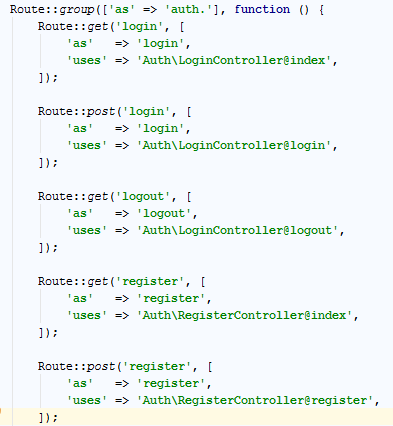
\includegraphics[height=2.5in]{Images/Implementation/LaravelRouting}
	\caption{A subset of the routes defined in the authentication} \label{fig:Routes}
\end{figure}

Figure \ref{fig:Routes} shows the code which defines all the routes regarding the different user authentication components. The routes are grouped together with a prefix using the \emph{'as'} parameter. This adds the 'auth::' prefix to the name of each route. For example, using \emph{route('auth::login')} will generate the URL pointing to the login page for user authentication. In addition to this, parameters can be included with the request for a route request, allowing for more flexible URLs. Included paramemters are passed to the relevant controller for the route. 

Routing with Laravel allows requests to be restricted to a certain type. With this, we can achieve security by limiting the type of HTTP request a route will accept. Laravel provides get, post, put, patch, and delete options for each route. A route defined using \emph{route::post} may only be accessed if the user posts form data to the URL. It is possible to bind a route to multiple request types such as get and post or even all request types but this is generally not recommended.

\subsection{Middleware}
HTTP middleware provides a convenient mechanism for filtering HTTP requests entering your application \cite{Laravel:Middleware}. Middleware is generally executed before a page is loaded in order to assess whether the user can access the page. It is possible to associate a page with multiple middlewares, and this can be thought of as a chain of middleware - requirements being passed from a previous middleware triggers a call to the next one. A middleware can be assigned to a route, method, controller or even a group of middleware.

It is possible to create custom middleware using the Artisan utility. The \textit{php artisan make:middleware Demo} command will generate a middleware called Demo. The image in figure \ref{fig:MiddlewareTemplate} shows the template that is generated by the Artisan utility. The commented block on line 17 can be replaced with a check, which if passed allows the next middleware to be activated but if failed returns an alternative action to be executed. Middleware was used in Fidelis to achieve several trivial tasks in the application, each of which are discussed in the relevant sections through the rest of this chapter.

\begin{figure}[H]
	\centering
	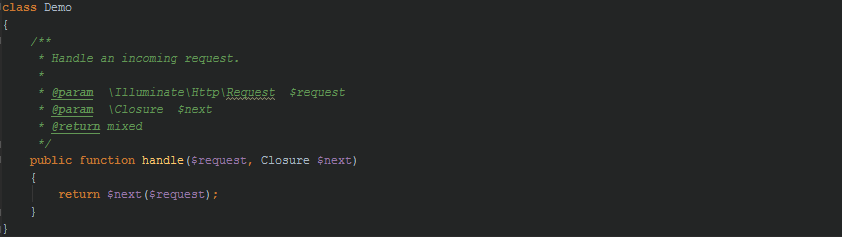
\includegraphics[height=2in]{Images/Implementation/MiddlewareTemplate}
	\caption{Middleware Template Generated by the Artisan Utility} \label{fig:MiddlewareTemplate}
\end{figure}

\section{Database}
The database is at the core of the application and thus care must be taken when setting up and configuring the database. A range of tools, provided by Laravel, were employed for configuring and interacting with the database. Details of the configuration and setup are discussed in detail.

\subsection{Configuration}
Database interactions occur through models, the query builder, schema builder and migrations provided as part of the Laravel framework. Settings inside the projects' configuration file must be tweaked in order for these components to function correctly. These settings allow the developer to change the connection, authentication and driver details for the application. In this project setup the PDO driver was used to connect to the database. Figure \ref{fig:DatabaseConfig} shows some of the settings that may be tuned in the configuration file.

\begin{figure}[H]
	\centering
	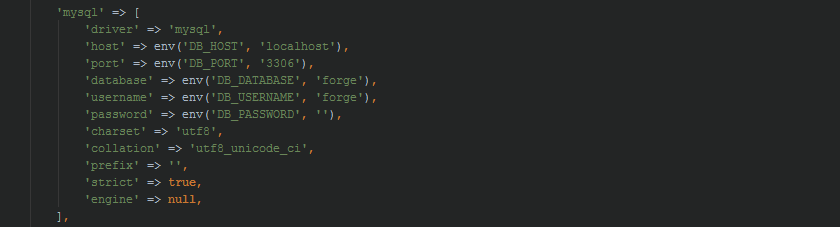
\includegraphics[height=2.3in]{Images/Implementation/MySQLConfig}
	\caption{Database Configuration for MySQL Databases} \label{fig:DatabaseConfig}
\end{figure}

\subsection{Migrations}
Migrations in Laravel are used to build database tables, and act as a database version control system, ``allowing a team to easily modify and share the application's database schema'' \cite{Laravel:Migrations}. The use of migrations not only allows for the database to be replicated anywhere the system is installed with ease but also simplifies the process of updating an existing table during the development process.  To create a migration, the \emph{make:migration}command provided by the Laravel Artisan utility is used. This command generates an empty template for a specified table. When creating a new table, the \emph{--create} argument is used whereas the \emph{--table} argument is used for modifying an existing table. The generated template contains an \emph{up} method, used for adding new columns and index, and a \emph{down} method which reverses the changes produced by the \emph{up} method. Migrations are typically paired with Laravel's schema builder to easily build your application's database schema \cite{Laravel:Migrations}. The schema builder can be used to define the schema for the table using calls to PHP functions. Once the schema has been populated, the \emph{migrate} command can be used to run the migration and update the database. In the case of an error the users can revert to a previous version of the database using the \emph{migrate:rollback} command. It is always encouraged that major changes, such as adding new columns and adding indexes, are introduced using new migrations rather than rolling back and updating existing migrations. All database tables were created using Laravel migrations and are available in the code.

\begin{figure}[H]
	\centering
	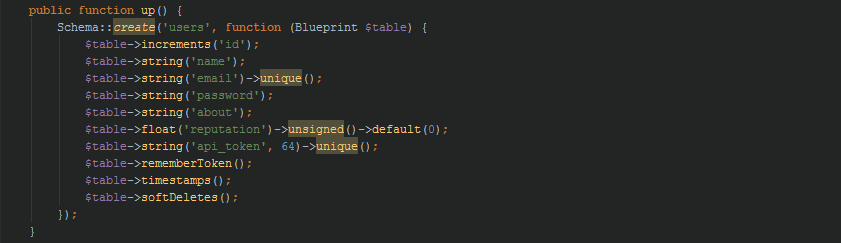
\includegraphics[height=2in]{Images/Implementation/UserMigration}
	\caption{Migration for creating Users table} \label{fig:UserMigration}
\end{figure}

Figure \ref{fig:UserMigration} shows the migration for the users table, which is used to store user information. The migration in the figure is not the final schema, and rather is the schema used during development. Additional migrations were used to add and modify columns in the table. As visible in the image, the schema builder can be used in the up method to define the structure of the table. Each migration schema contains an \emph{id} field, generated by calling the \emph{increments} method, and the \emph{created\_at} and \emph{updated\_at} timestamps, generated by calling the \emph{timestamps} method, by default. The \emph{increments} method is used for assigning an auto incrementing primary key, discussed later in the report, used for associating record through relationships. A \emph{deleted\_at} timestamp was added to all tables by calling the \emph{softDeletes} method. A range of other method such as \emph{string} and \emph{integer} can be used for creating more attributes. A full list of operations is available in the Laravel documentation \cite{Laravel:Migrations}. 

\subsection{Functional Dependencies and Constraints}
Majority of the foreign key constraints used in the database were setup with cascade delete and cascade update. This means that if a row in the referenced entity is removed or updated then any rows in the referencing entity which correspond to it are also updated or deleted \cite{TechOnTheNet:Cascading}. Some of the constraints followed the schema-bound dependencies by using the restrict keyword which prevents changes in the referenced entity if corresponding rows exist in the referencing entity. The use of all these techniques ensures that data is always kept consistent and no redundant data is introduced into the system.

\subsection{Security}
Security is of the upmost importance when it comes to a database which contains sensitive or personal information about individuals. For this reason, several measures should be taken into consideration to protect the database and the data in it from unauthorised access. The security threats and approaches taken to protect against them are discussed below.

\subsubsection{Access}
The first step to protecting the data is controlling who has access to the database and who is authorised to do what. This was achieved by creating separate SQL user accounts with different privileges. The database was then protected using a password to prevent any unauthorised access and only authorised users with a username and password would be able to access the database. Furthermore, each user was restricted so that the database would accept connections from the user if they were from a specified IP address. This meant that database connections could be restricted to just the web server and any users attempting to connect to the database from other machines would be denied access. When connecting to the database through PHP, root account was used for development purposes to prevent any restrictions but a separate account was used for production which was unable to modify the schema but could still query or modify the data.

\subsubsection{SQL Injection}
``SQL injection is a technique where malicious users can inject SQL commands into an SQL statement, via web page input'' \cite{W3Schools:SQL_Injection}. According to a report on 5,500 companies and 15,000 websites, almost half of these were vulnerable to serious security threats by XSS or SQL injection \cite{FirstPost:Vulnerabilities}. SQL injection can lead to all the data held in a database being made available. This is a serious threat as some of the data can be used to identify individuals and measures should be introduced to protect against this. One way to prevent SQL injection is by escaping all user input to prevent users from executing malicious queries. This is not a full fix for the issue as users can still enter data that can cause the system to malfunction. The alternative fix for this was using prepared queries which executes the query with placeholders and then binds the values later to retrieve the records. This method escapes SQL injection and prevents any unauthorised interaction with the database.

\subsection{Querying}
Laravel makes running queries extremely simple using either raw SQL statements, the fluent query builder, or the Eloquent Object-Relational Mapping (ORM) \cite{Laravel:Database}. For most part the Eloquent ORM approach was used to retrieve the result from the database but the approaches have been used in rare cases. All three approaches are outlined below.

\paragraph{Raw SQL}
With Laravel, raw SQL statements can be executed using the provided built-in classes. This removes the need to open a database connection, create SQL statements and bind parameters to these statements as this is all done automatically. For example, as shown in the example below, the user can run an SQL query to retrieve a user with a specific ID of 1 just by using the \emph{DB::select} method:

\begin{lstlisting}[language=php]
	$users = DB::select('SELECT * FROM users WHERE id = ?', [1]);
\end{lstlisting}

\noindent The above query will return an array of objects modelling the user entity in the database. Using this array, it is possible to loop through the array and access the properties of each user as \emph{\$user-$>$property}, where property may be any attribute such as username or email.

\paragraph{Query Builder}
The database query builder provides a convenient, fluent, and easy-to-use interface for creating and executing database queries \cite{Laravel:QueryBuilder}. The query builder can perform most operations supported by the database driver. One of the main advantages of using the query builder is that it uses PDO parameter bindings to prevent SQL injections, which means there is no need to sanitise user input. Using the query builder, one could retrieve the user with ID 1 by executing the following statement:

\begin{lstlisting}[language=php]
	$user = DB::table('users')->where('id', 1)->first();
\end{lstlisting}

\noindent The above query would fetch the result where the user ID matches the provided parameter and retrieve the first result. Once again, the result is returned as an object modelling the user entity and the properties can be accessed again as \emph{\$user-$>$property}.

\paragraph{Eloquent Object-Relational Mapping}
The Eloquent ORM included with Laravel provides an simple and elegant active record implementation for working with the database \cite{Laravel:Eloquent}. "Object-relational mapping (ORM) is a mechanism that makes it possible to address, access and manipulate objects without having to consider how those objects relate to their data sources" \cite{TechTarget:ORM}. Each database table has a corresponding "model" associated with it that is used database interactions and more specifically the table corresponding to a given model. Models allow the developer to query, insert, update, and delete records in the corresponding table as well as more complex operations such as joining tables. When querying the database using a model, Eloquent automatically instantiates and maps a model for each row in the result allowing the developer to utilise the models behaviour.

\begin{lstlisting}[language=bash]
	$ php artisan make:model Models/User
\end{lstlisting}

\noindent Creating a model is made simple again thanks to the Artisan utility. The command above will generate a User model in the \emph{app/Models} directory. Each Eloquent models extends the \emph{Illuminate/Database/Eloquent/Model} class which utilises the query builder for all interactions \cite{Laravel:Eloquent}. By default, Eloquent assumes that each table has a primary key field named \emph{id} and the \emph{created\_at} and \emph{updated\_at} timestamps but these can all be changed by toggling optional properties in the model. In order to use a model, the developer simply needs to import the model in the controller where it will be used. The user can simple execute the following command in order to retrieve the user with ID=1.

\begin{lstlisting}[language=php]
	$user = User::find(1);
\end{lstlisting}

\noindent The line of code above will return the \emph{User} model. It is again possible to access the model properties as \emph{\$user-$>$property}. The main change to be noticed here is that the user can actually update the properties and save the changes made by executing the following: \emph{\$user-$>$save()} \cite{Laravel:Eloquent}.  The image in figure \ref{fig:UserModel} shows the code for the \emph{User} model. As visible in the image, it is possible to add custom methods to the model which may be called when the model is returned as a result.

\begin{figure}[H]
	\centering
	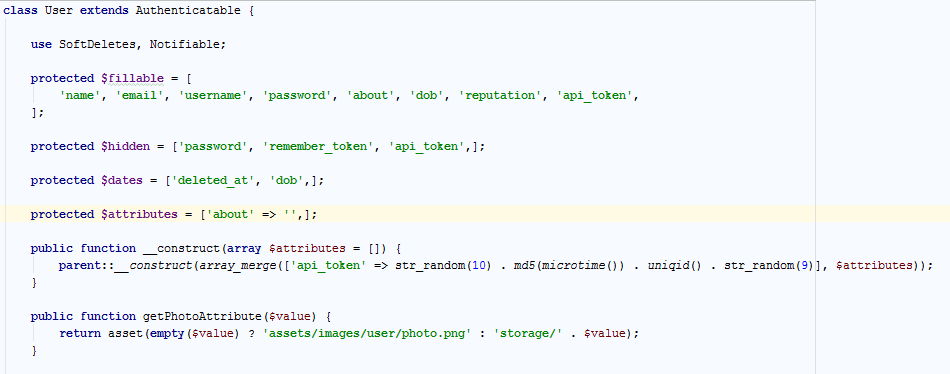
\includegraphics[width=1.0\textwidth]{Images/Implementation/UserModel}
	\caption{Users Eloquent ORM model} \label{fig:UserModel}
\end{figure}

\section{Data Collection}
Although some of the data will be collected through manual inputs and downloading readily available resources from Kaggle, further data will be required to be collected using API services from social networks such as Twitter. In this section, the implementation of collecting the data from these API services is discussed, as well as how data from manual input is transferred to storage for use by Fidelis.

\subsection{Training Data}
For the abuse detection training data, the data is downloaded as a CSV file from Kaggle which is ready to be used for training the machine learning model ~\cite{Kaggle:Dataset}. However, for the content filtering model, the dataset from Zubiaga and Ji needs manipulating so that the Tweet's text can be used for training ~\cite{Zubiaga:Tweets}. The downloaded dataset only provides the Tweet ID, therefore this ID can be used to collect the relevant Tweet text from the Twitter API via the Python library Tweepy ~\cite{Tweepy}.

To collect the relevant Tweets from the API, a Python script was used, which reads in the original dataset and, for all of the Tweets, requests the Tweet from the Twitter API based on the Tweet ID, before writing the Tweet text, along with the category from the original dataset, to a new CSV file. All interactions with the Twitter API were handled using the Tweepy Python library ~\cite{Tweepy}. 

\subsubsection{OAuth}
To gain access to the Twitter API, OAuth is used to authenticate whether or not a user is allowed to view content via the API. Figure \ref{fig:oauth} below shows how the OAuth handshake is implemented in Tweepy. The \textit{consumer\_token} and \textit{consumer\_token\_secret} values are obtained from Twitter when you create an application for Twitter. The URL produced by \textit{get\_authorization\_url()} is a link which the user follows in order to grant access to the application to the user's Twitter account. Twitter then produces the user's request token which can be used to retrieve the user's access token and access token secret for the application, which are printed at the end of the script. Once the application has these, it can then make requests on behalf of the user to the Twitter API.

\begin{figure}[H]
	\centering
	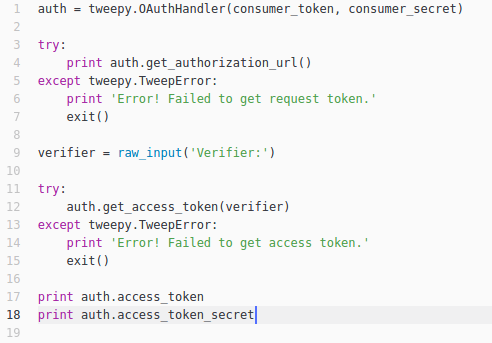
\includegraphics[height=2in]{Images/Implementation/oauth}
	\caption{Twitter OAuth handshake} \label{fig:oauth}
\end{figure}

\subsubsection{Querying the API}
Once the access token and access token secret has been obtained, a Tweepy API object can be made, which allows the application to make queries to the Twitter API. This script can iterate over each Tweet ID and retrieve the Tweet in order to collect the Tweet text, as shown in figure \ref{fig:get-tweets}. The output of the script can then be saved as the new dataset CSV, with the Tweet IDs replaced by the Tweet text.

\begin{figure}[H]
	\centering
	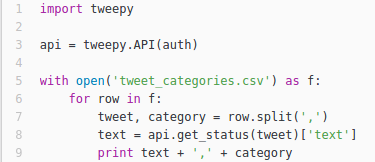
\includegraphics[height=1in]{Images/Implementation/get-tweets}
	\caption{Get Tweet from API} \label{fig:get-tweets}
\end{figure}

\subsubsection{Virtual Private Servers}
Due to the size of the training set and the rate limits imposed by Twitter on their API, the amount of time it would take to process the entire original dataset to collect the Tweet text would be significant. To mitigate this, multiple access tokens can be used simultaneously on separate VPS's, by dividing the dataset amongst the servers and running the script remotely, since the rate limits are imposed on each access token rather than each application. For the purposes of this task, the CentOS Digital Ocean droplet can be used ~\cite{DigitalOcean:Home}. Although the amount of storage on the droplet means that the entire dataset can not be processed, even when dividing amongst 10 access tokens, it allows a large enough dataset to be produced within a reasonable time frame.

\subsection{Template Data}
The template data can be simply added to the Laravel database using the migration seeds. Figure \ref{fig:seed} shows the user seed file, which adds the template data for the user table to the database through the User model. Each attribute in the User model corresponds with a column on the users table. To add the seeds into the table, the Artisan command \textit{php artisan db:seed} is run.

\begin{figure}[H]
	\centering
	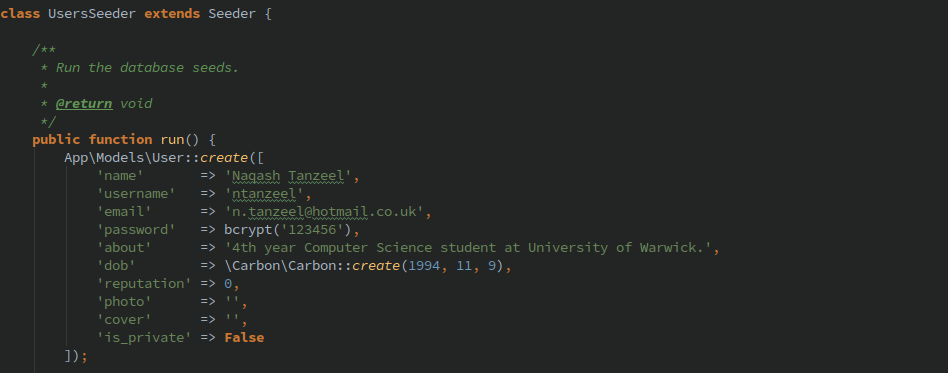
\includegraphics[height=3in]{Images/Implementation/seed}
	\caption{User Seed} \label{fig:seed}
\end{figure}

\subsection{User Authentication}
The form shown in figure \ref{fig:register-page} is used to collect the data needed in order to authenticate access for the user, which includes the password fields and also the email address so that a password can be recovered in case it is forgotten by the user. When this form is submitted, the form data is passed to the RegisterController.php, which handles adding the user to the database via the User model. The function which performs this process is shown in figure \ref{fig:register-controller}.

\begin{figure}[H]
	\centering
	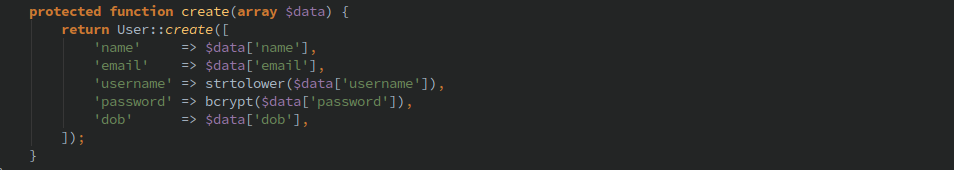
\includegraphics[height=1.5in]{Images/Implementation/register-controller}
	\caption{Register Controller} \label{fig:register-controller}
\end{figure}

\section{Data Processing}
As mentioned earlier, Python was chosen for data processing. Python has an established data analysis community, and as such provides a rich assortment of open-source libraries that can be used. With a such a community, documentation was abundant and meant that the implementation of the designs discussed in Chapter \ref{Chapter:Design} were accelerated greatly. Not only this, but existing solutions for problems encountered during development were available, which again sped up the implementation process. 

\subsection{Abuse Detection}
\subsection{Content Filtering}
The implementation of content filtering constitutes of Python scripts which handle all of the data preprocessing, training of the model and predicting of the post categories. As with abuse detection, this makes use of multiple Python libraries including Sci-kit learn \cite{scikit:home}, NLTK \cite{nltk}, Numpy \cite{Numpy} and Pandas \cite{Pandas}, which provide machine learning models and objects for processing datasets. The code is divided between three files, each of which handle a stage of the machine learning process: preprocess.py, training.py and predict.py.

\subsubsection{Data Preprocessing}
The file preprocess.py cleans the textual post so that it can be passed onto either the training or predicting processes.

\subsubsection{Model Building}

\subsubsection{Predicting Topics}

\subsection{Content Recommendation}
Content recommendations are generated from a single python script. It was decided to go with a single script as certain techniques are shared between user and post recommendations. The script is modularised by using functions that enable code blocks to be re-used. Python list comprehension provides a succinct way to generate lists \cite{Python:ListComprehension}, and this syntax is used throughout implementation.

Before recommendations can be made, a database connection is established using the mysql.connector library, ``a Python driver for communicating with MySQL servers'' \cite{MySQL:MySQLConnector}. This library contains a number of useful functions for database interactions. Recommendation generation only occurs if the attempt to connect to the database is successful, otherwise an error message is logged. This prevents erroneous system behaviour. To begin recommendations, all users are first retrieved from the database. To tailor recommendations to a specific user, user settings for how they want their recommendations to be generated are retrieved. Default settings are set for new users but these can be changed on the settings page. The settings retrieved are for recommendation preference (FOF, Explorer or Hybrid recommendations), the number of recommendations to generate, recommendation threshold (for vector similarity) and recommendation reputation. Figure \ref{fig:RecommendationSettings} shows how user settings are retrieved.


\begin{figure}[H]
\centering
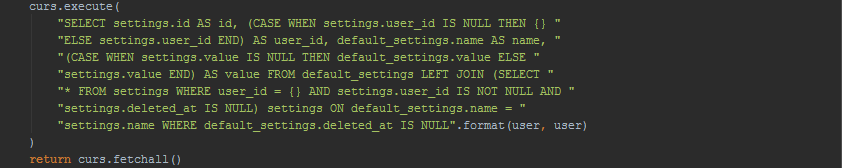
\includegraphics[height=2in]{Images/Implementation/RecommendationSettings}
\caption{Function that executes query for retrieving user settings}
\label{fig:RecommendationSettings}
\end{figure}

\noindent Letting the use have control over this settings will allow them to fine-tune how they want to receive recommendations. The next two sections will look at how user and post recommendations are generated.

Recommendations are generated using either FOF, Explorer or Hybrid users. The technique chosen for generation is dependent on the preference set by the user. To begin with, a query retrieving a count of the number of user recommendations already generated for the user is retrieved. New recommendations are only made if this count is less than the number of recommendations specified by the user. We will now look at how each of these techniques are implemented. Processes will be discussed for an individual user, who we will refer to as the recommendee, but each is repeated for all users stored in the database.

\subsubsection{Friend-of-a-Friend Recommendations}
FOF candidate recommendations are retrieved by first getting all users followed by the recommendee. These users are looped through, and for each of them the users they follow are collected and appended to a list. The recommendee is excluded from this list. Once this list has been generated, it is flattened to become a single list, which we will refer to as the \textit{fof\_users} list.

\paragraph{User} From this list, FOF user recommendations are chosen by converting the list to a Counter object and picking the most common elements. The counter object was used for this purpose as it enables quick tallying \cite{Python:Counter} the \texttt{most\_common()} method on Counter objects accepts a parameter value for the number of common elements to be returned. This ensures that only the number of required recommendations for the recommendee are returned. Use of the Counter object is given below:

\begin{lstlisting}[language=python]
	fof_users = Counter(fof_users).most_common(num_recommendations)
\end{lstlisting}

Reasoning for not using cosine similarity between candidate recommendations and the recommendee are given in Chapter \ref{Chapter:Design}.

\paragraph{Post} Using the same technique for post recommendations, the users in the \textit{fof\_users} list are looped through, retrieving the posts made by each of the  users. For a post to suffice as a candidate recommendation for the recommendee, its reputation is compared with the reputation threshold set by the recommendee. If the reputation of the post exceeds the threshold, it is returned as one of the posts in the list of recommendations for the recommendee.

\begin{figure}[H]
\centering
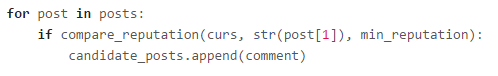
\includegraphics[height=0.7in]{Images/Implementation/FOFPostReputation}
\caption{Code for assessing the reputation of a candidate post recommendation}
\label{fig:FOFPostReputation}
\end{figure} 

\noindent Figure \ref{fig:FOFPostReputation} shows the process for comparing the reputation of a candidate post recommendation with the minimum reputation set by the user. Performing this check ensures again that recommendations being made are tailored to the recommendee's preferences.

\subsubsection{Explorer Recommendations}
Explorer recommendations make use of the recommendee's `tag count vector', which is a vector representing the number of posts the recommendee has made in each of the available tags. The vector is generated by first creating a zero-filled list which has a length equal to the number of tags currently stored. Each entry in the list is a (TagID, Count) tuple. This list, which we shall refer to as the recommendee\_vector is then sorted to determine the recommendee's favourite tags to post in. Candidate recommendations are retrieved from these tags. Currently, there is no cap on the number of tags looked at, but a cap on the number of ``favourite tags'' can be set once the system grows beyond what is considered small. The recommendee's favourite tags are looped through, retrieving other users posting in the same tag. This is shown in Figure \ref{fig:ExplorerFavouriteTags}.

\begin{figure}[H]
\centering
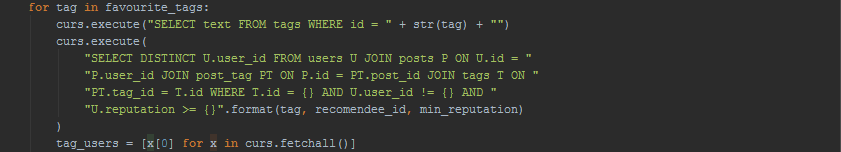
\includegraphics[height=2in]{Images/Implementation/ExplorerFavouriteTags}
\caption{Code for retrieving users who post in the recommendee's preferred tags}
\label{fig:ExplorerFavouriteTags}
\end{figure}

\paragraph{User} Explorer user recommendations are assessed based on the similarity between a tag user (user also posting in one of the recommendee's preferred tags) and the recommendee. Similarity is measured using cosine similarity. SciPy provides a number of distance computation functions, one of which the cosine distance. This is used to measure the distance between the vector generated for the tag user and the recommendee's vector. To get similarity from this, the result of this measurement is subtracted from one.

\begin{figure}[H]
\centering
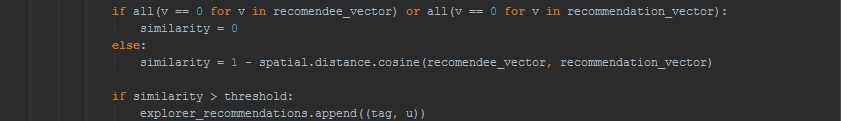
\includegraphics[height=2in]{Images/Implementation/ExplorerSimilarity}
\caption{Measuring similarity between users for Explorer recommendations}
\label{fig:ExplorerSimilarity}
\end{figure}

\noindent In Figure \ref{fig:ExplorerSimilarity}, we see that we need to account for a user vector containing all zeros. This is possible for new or existing users who have made no posts. To account for this, similarity is only measured if neither of the two user vectors contain only zeros. Once similarity is measured, it is compared with the threshold for similarity set by the user. Only users with a similarity that exceeds this threshold are given as recommendations. In the figure we can see again that recommendations are saved as (TagID, Before the set of user recommendations is returned, its length is compared with the number of recommendations needed to provide only the required number of recommendations. 

\paragraph{Post} Similarly to post recommendations generated using the FOF technique, posts made by each of the tag users are retrieved. Only those exceeding the reputation set by the recommendee are given as recommendations. Akin to user recommendations, only the number of required recommendations are returned.

\subsubsection{Hybrid Recommendations}
Hybrid recommendations are generated by finding the intersection between the recommendations made using the FOF and Explorer recommendation methods. The Python Standard Library provides a \textit{sets} module, which can create a set of unordered, unique elements from a list \cite{Python:Sets}. Using this module, it is possible to convert the lists returned from each of the recommendation methods to sets and find the intersection between the two. We can see this in Figure \ref{fig:HybridRecommendations}.

\begin{figure}[H]
\centering
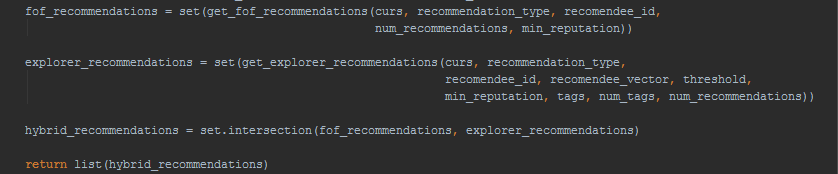
\includegraphics[height=1.5in]{Images/Implementation/HybridRecommendations}
\caption{Generation of hybrid recommendations}
\label{fig:HybridRecommendations}
\end{figure}

\subsubsection{Default Recommendations}
In the event that all previous methods for generating recommendations fail, the script reverts to a default method that will generate generic recommendations for the recommendee. 

\paragraph{User} Generic user recommendations will consist of users with the highest reputation in the system. To further filter this, only users with a reputation greater than the minimum reputation set by the user are returned.

\begin{figure}[H]
\centering
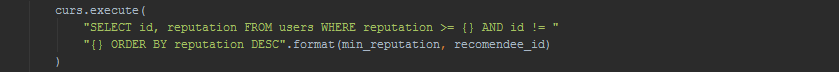
\includegraphics[height=0.7in]{Images/Implementation/DefaultUsers}
\caption{Query for selecting most reputable users}
\label{fig:DefaultUsers}
\end{figure}

\paragraph{Post}
Similarly to users, default post recommendations are made based off the most reputable posts in the system.

\begin{figure}[H]
\centering
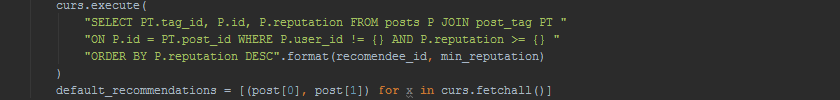
\includegraphics[height=1in]{Images/Implementation/DefaultPosts}
\caption{Query for selecting most reputable posts}
\label{fig:DefaultPosts}
\end{figure}

\subsubsection{Cleaning and Saving Recommendations}
Once recommendations have been generated, they need to be cleaned. The first step in cleaning involves removing any recommendations the user currently has and has not responded to. In addition to this, cleaning user recommendations consists of:
\begin{itemize}
\item Removing blocked users
\item Removing users the recommendee already follows
\item Removing the recommendee themselves
\end{itemize}

\noindent Cleaning post recommendations consists of:
\begin{itemize}
\item Removing posts made by users the recommendee has blocked
\item Removing posts the recommendee has voted on and therefore has already seen
\end{itemize}

In the case of cleaning post recommendations, posts made by the recommendee are not removed as all queries involving candidate post recommendations omit posts made by the recommendee.

Once recommendations have been cleaned, new recommendations are inserted into the relevant table. After storing the recommendations, changes made to the database must be committed using the \texttt{commit()} function on the connection object.

\subsection{Reputation Scoring}

\section{User Interface}
\subsection{Navigation}
\subsection{Authentication}
\subsubsection{Registration}
\subsubsection{Login}
\subsubsection{Recover Account}
\subsubsection{Authorised Access}
\subsection{Home}
\subsection{Discover}
\subsection{Notifications}
\subsection{Profile}
\subsection{Settings}
\subsection{Static Pages}
\subsubsection{Privacy Policy}
\subsubsection{Support}